%%%%%%%%%%%%%%%%%%%%%%%%%%%%%%%%%%%%%%%%%%%%%%%%%%%
%
%  New template code for TAMU Theses and Dissertations starting Fall 2012.  
%  For more info about this template or the 
%  TAMU LaTeX User's Group, see http://www.howdy.me/.
%
%  Author: Wendy Lynn Turner 
%
%%%%%%%%%%%%%%%%%%%%%%%%%%%%%%%%%%%%%%%%%%%%%%%%%%%

\documentclass[12pt]{report}
\usepackage[letterpaper]{geometry}
\geometry{verbose,tmargin=1.25in,bmargin=1.25in,lmargin=1.4in,rmargin=1.15in}
 \usepackage[doublespacing]{setspace}
 \usepackage{tocloft}
 \usepackage[rm, tiny,center, compact]{titlesec}
 \usepackage{indentfirst}
 \usepackage{etoolbox}
\usepackage{tocvsec2}
 \usepackage[titletoc]{appendix}
 \usepackage{appendix}
% \usepackage{tamuconfig}
 \usepackage{pvamuconfig}
\usepackage{rotating}

% Added to fix issues with pdf searching in some versions of LaTeX
%\usepackage[T1]{fontenc}\usepackage{lmodern}
%%%%%%%%%%%%%%%%%%%%%%%%%%%%%

\usepackage{listings}

\usepackage{color}
\definecolor{gray}{rgb}{0.4,0.4,0.4}
\definecolor{darkblue}{rgb}{0.0,0.0,0.6}
\definecolor{cyan}{rgb}{0.0,0.6,0.6}

\lstset{
  basicstyle=\ttfamily,
  columns=fullflexible,
  showstringspaces=false,
  commentstyle=\color{gray}\upshape
}

\lstdefinelanguage{XML}
{
  morestring=[b]",
  morestring=[s]{>}{<},
  morecomment=[s]{<?}{?>},
  stringstyle=\color{black},
  identifierstyle=\color{darkblue},
  keywordstyle=\color{cyan},
  morekeywords={xmlns,version,type}% list your attributes here
}

\usepackage{pbox}

\usepackage{caption}
\usepackage{subcaption}
\usepackage{breakcites}
\usepackage{url}
\usepackage{tabularx}

\usepackage{array}
\newcolumntype{L}[1]{>{\raggedright\let\newline\\\arraybackslash\hspace{0pt}}m{#1}}
\newcolumntype{C}[1]{>{\centering\let\newline\\\arraybackslash\hspace{0pt}}m{#1}}
\newcolumntype{R}[1]{>{\raggedleft\let\newline\\\arraybackslash\hspace{0pt}}m{#1}}

\usepackage{textcomp}

% Hyperref setup below.  You should be able to get away with using uncommenting just the first line.
%\usepackage[hidelinks]{hyperref}

% if \usepackage[hidelinks]{hyperref} doesn't work try this.
% \usepackage{hyperref}  % Hidelinks is an option that removes link visiability.  TAMU Thesis Offices prefers to not see the links. But often doesn't work.  
% 
% \hypersetup{
%     colorlinks=true,
%     linkcolor=black,
%     citecolor=black,
%     filecolor=black,
%     urlcolor=black,
% }
%%%%%%%  End of hyperref setup.  One of these two options should work, but my motto with hyperref is when in doubt, comment it out!
%%%%%%%%%  This hopefully fixes the problem with vertical spacing of section headings at the top of the page..  Commented out in 1.0.7
% \preto\section{%
% \ifnum\value{section}>0\addtocontents{toc}{\vskip-6pt}\fi
% }
% \preto\subsection{%
% \ifnum\value{subsection}=0\addtocontents{toc}{\vskip-6pt}\fi
% \ifnum\value{subsection}>0\addtocontents{toc}{\vskip-6pt}\fi
% } 
%%%%%%%%%%%%%%%%%%%%%%%%%%%%%%%%%%%%%%%%%%%%%%%%%%%%%%

\begin{document}

% Change to PVAMU format
\ifx true false 
\renewcommand{\tamumanuscripttitle}{A Scalable and Distributed Seismic Data Toolkit on Big Data Analytics Platform}
\renewcommand{\tamupapertype}{Dissertation}
\renewcommand{\tamufullname}{Chao Chen}
\renewcommand{\tamudegree}{Master Degree}
\renewcommand{\tamuchairone}{Dr. Lei Huang}
% Uncomment out the next line if you have co-chairs.  You will also need to edit the titlepage.tex file.
%\newcommand{\tamuchairtwo}{Additional Chair Name}
\renewcommand{\tamumemberone}{Dr. Lei Huang}
\newcommand{\tamumembertwo}{Dr. Lin Li}
\newcommand{\tamumemberthree}{Dr. Sherri S. Frizell}
\renewcommand{\tamudepthead}{Dr. Yonggao Yang}
\renewcommand{\tamugradmonth}{December}
\renewcommand{\tamugradyear}{2016}
\renewcommand{\tamudepartment}{Department of Computer Science}
\fi

\renewcommand{\pvamucollege}{PRAIRIE VIEW A\protect\&M UNIVERSITY\protect\\COLLEGE OF ENGINEERING\protect\\PRAIRIE VIEW, TEXAS}
\renewcommand{\pvamumanuscripttitle}{A Scalable and Distributed Seismic Data Toolkit on Big Data Analytics Platform}
\renewcommand{\pvamupapertype}{Thesis}
\renewcommand{\pvamusubmitto}{Submitted to the Graduate School\\In Partial Fulfillment of the Requirements for\\The Degree of}
\renewcommand{\pvamudegree}{MASTER OF SCIENCE}
\renewcommand{\pvamumajor}{COMPUTER SCIENCE}
\renewcommand{\pvamufullname}{Chao Chen}
\renewcommand{\pvamuadvisor}{Advisor Name}
\renewcommand{\pvamudepthead}{Department Head}
\renewcommand{\pvamucollegedean}{College Dean Name}
\renewcommand{\pvamugraddean}{Graduate School Dean Name}
\renewcommand{\pvamugradmonth}{December}
\renewcommand{\pvamugradyear}{2016}


%\include{titlepage} % This is simply a file that formats and adds your titlepage, please do not edit this unless you have a specific need. .
%%%%%%%%%%%%%%%%%%%%%%%%%%%%%%%%%%%%%%%%%%%%%%%%%%%
%
%  New template code for TAMU Theses and Dissertations starting Fall 2012.  
%  For more info about this template or the 
%  TAMU LaTeX User's Group, see http://www.howdy.me/.
%
%  Author: Wendy Lynn Turner 
%	 Version 1.0 
%  Last updated 8/5/2012
%
%%%%%%%%%%%%%%%%%%%%%%%%%%%%%%%%%%%%%%%%%%%%%%%%%%%

%%%%%%%%%%%%%%%%%%%%%%%%%%%%%% 
%% TITLE PAGE
%% The values get updated automatically.  Please do not make changes to this file other than adding/deleting committee members where necessary.
%%%%%%%%%%%%%%%%%%%%%%%%%%%%%%

\begin{titlepage}
\begin{center}

\vspace*{50 pt}
%\providecommand{\tabularnewline}{\\}
\MakeUppercase{\pvamumanuscripttitle}

\vspace{60 pt}
A \pvamupapertype

by

\MakeUppercase{\pvamufullname}

\vspace{60 pt}

\begin{singlespace}
Submitted to the Office of Graduate Studies of \\
Prairie View A\&M University \\
in partial fulfillment of the requirements for the degree of\\
\end{singlespace}

\vspace{20 pt}
\MakeUppercase{\pvamudegree}

\vspace{60 pt}

%\begin{center}
\pvamugradmonth \hspace{2pt} \pvamugradyear
%\par\end{center}

\vspace{60 pt}

Major Subject: Computer Science
\par\end{center}

\end{titlepage}
\pagebreak{}





%%%%%%%%%%%%%%%%%%%%%%%%%%%%%%%%%%%%%%%%%%%%%%%%%%%
%
%  New template code for TAMU Theses and Dissertations starting Fall 2012.  
%  For more info about this template or the 
%  TAMU LaTeX User's Group, see http://www.howdy.me/.
%
%  Author: Wendy Lynn Turner 
%	 Version 1.0 
%  Last updated 8/5/2012
%
%%%%%%%%%%%%%%%%%%%%%%%%%%%%%%%%%%%%%%%%%%%%%%%%%%%
%%%%%%%%%%%%%%%%%%%%%%%%%%%%%%%%%%%%%%%%%%%%%%%%%%%%%%%%%%%%%%%%%%%%%
%%                           ABSTRACT 
%%%%%%%%%%%%%%%%%%%%%%%%%%%%%%%%%%%%%%%%%%%%%%%%%%%%%%%%%%%%%%%%%%%%%

\chapter*{ABSTRACT}
\addcontentsline{toc}{chapter}{ABSTRACT} % Needs to be set to part, so the TOC doesnt add 'CHAPTER ' prefix in the TOC.

\pagestyle{plain} % No headers, just page numbers
\pagenumbering{roman} % Roman numerals
\setcounter{page}{2}

\begin{center}
\pvamumanuscripttitle

\pvamugradmonth \hspace{2pt} \pvamugradyear

\pvamufullname, B.S., southwest university of science and technology;

Chair of Advisory Committee: Dr. Lei Huang 

\par\end{center}

\indent Seismic volume is a basic data structure that has been widely used in geophysical computing, as well as in big data analytics applications of petroleum industry. It has been well studied in High Performance Computing (HPC) platforms. However, a little study has been done in big data analytics platforms. In this paper, we present an efficient Distributed Seismic Data Analytics Toolkit that works on the popular Apache Spark big data analytics platform. The toolkit supports different ways of seismic volume data distributions, repartition, transposing, access, and data parallelism with a variety of parallel execution templates. This work studies the performance characteristics of these seismic volume data operations with different configurations, current status of this big data analytics cloud at PVAMU as well as our research plan for future work. The scalability and parallelism are the main characteristics of this platform.  


 

\pagebreak{}

%\include{dedication}
%%%%%%%%%%%%%%%%%%%%%%%%%%%%%%%%%%%%%%%%%%%%%%%%%%%
%
%  New template code for TAMU Theses and Dissertations starting Fall 2012.  
%  For more info about this template or the 
%  TAMU LaTeX User's Group, see http://www.howdy.me/.
%
%  Author: Wendy Lynn Turner 
%	 Version 1.0 
%  Last updated 8/5/2012
%
%%%%%%%%%%%%%%%%%%%%%%%%%%%%%%%%%%%%%%%%%%%%%%%%%%%


%%%%%%%%%%%%%%%%%%%%%%%%%%%%%%%%%%%%%%%%%%%%%%%%%%%%%%%%%%%%%%%%%%%%%%
%%                           ACKNOWLEDGEMENTS
%%%%%%%%%%%%%%%%%%%%%%%%%%%%%%%%%%%%%%%%%%%%%%%%%%%%%%%%%%%%%%%%%%%%%
\chapter*{ACKNOWLEDGEMENTS}
\addcontentsline{toc}{chapter}{ACKNOWLEDGEMENTS}  % Needs to be set to part, so the TOC doesnt add 'CHAPTER ' prefix in the TOC.

I would like to thank my advisor, professors, colleagues and friends who helped me a lot in the past two years. I cannot make it through and finish my thesis without their kind help.

First I want to thank my advisor Dr. Lei Huang, for giving me the chance to work in CloudComputing Lab and guiding my study and research in cloud computing, and thanks to Dr. Lin Li and Dr. Frizell for spending their time to refine my thesis which benefits me a lot in academic writing skills. Special thanks to Mr Ted Clee, for sharing his deep knowledge of seismic data analytics.

I also appreciate all my colleagues and classmates worked in the lab in the past two years, for sharing so many interesting things from different cultures, and, of course, for helping and encouraging each other in research work.

Last but not least, I want to thank my friend Yuzhong Yan, for always being the guy helps me out at so many tough time in my life. I have learned so much from him not only as an engineer but also as a kind and wise man. 

\pagebreak{}

\ifx true false
\vspace*{\fill}
\begin{center}
A.M.D.G.
\end{center}
\vspace*{\fill}
\pagebreak{}
\fi

%\include{nomenclature}

\include{lists}  % This is simply a file that formats and adds your toc, lof, and lot, please do not edit this unless you have a specific need. .

%%%%%%%%%%%%%%%%%%%%%%%%%%%%%%%%%%%%%%%%%%%%%%%%%%%
%
%  New template code for TAMU Theses and Dissertations starting Fall 2012.  
%  For more info about this template or the 
%  TAMU LaTeX User's Group, see http://www.howdy.me/.
%
%  Author: Wendy Lynn Turner 
%	 Version 1.0 
%  Last updated 8/5/2012
%
%%%%%%%%%%%%%%%%%%%%%%%%%%%%%%%%%%%%%%%%%%%%%%%%%%%

%%%%%%%%%%%%%%%%%%%%%%%%%%%%%%%%%%%%%%%%%%%%%%%%%%%%%%%%%%%%%%%%%%%%%%
%%                           SECTION I
%%%%%%%%%%%%%%%%%%%%%%%%%%%%%%%%%%%%%%%%%%%%%%%%%%%%%%%%%%%%%%%%%%%%%


\pagestyle{plain} % No headers, just page numbers
\pagenumbering{arabic} % Arabic numerals
\setcounter{page}{1}


\chapter{\uppercase {Introduction}}

\section{Background}
Petroleum is a traditional industry where massive seismic data sets are acquired for exploration using land-based or marine surveys. Huge amount of seismic data has already been generated and processed for several decades in the industry, although there was no big data concept at that time. High Performance Computing (HPC) has been heavily used in the industry to process the pre-stack seismic data in order to create 3D seismic property volumes for interpretation. 

Currently, reflection seismology (or seismic reflection) is the most important method used in the petroleum industry to estimate the properties of the Earth's subsurface from reflected seismic waves and explore geophysics using the principles of seismology. The complete processing flow of this method involves data acquisition, data processing, data interpretation and attributes analysis \cite{seisreflectionwiki}. 

As shown in Figure \ref{seismic_reflection}, data acquisition is performed by using seismic sources such as dynamite or air gun generate to spread out seismic waves, which are reflected back from encountered materials underground and then recorded by the receiving sensors. To get data-scientists-usable 2D/3D seismic dataset, the collected seismic wavelet needs to be pre-processed by data processing methods including deconvolution, common-midpoint (CMP) stacking and migration. After data processing, the seismic events are geometrically re-located in either space or time to the location the event occurred in subsurface and create a complete image of subsurface \cite{seisreflectionwiki}. 

The goal of seismic data interpretation and  attributes analysis is to locate the potential petroleum reservoirs from processed seismic reflections map. It involves deep knowledge of seismic attributes, geophysics, and intensive collaborations between data scientists and geophysicists. This thesis focus on develop a scalable and distributed toolkit to facilitates seismic data attributes analytics.   

\begin{figure}[h]
\centering
\includegraphics[scale=0.4]{figures/seismic_reflection_principal.png}
\caption{Reflection Seismology \cite{seisreflectionepa} \cite{seisreflectionagile}}
\label{seismic_reflection}
\end{figure}

%A landscape figure should be shown below. 
%%%%%%%%%%%%%%%%%%%%%%%%%%%%%%%%%%%%%%%%%%%%%%%%%%%%%%
%\begin{sidewaysfigure}[H]
%\centering
%\includegraphics[scale=.50]{figures/Penguins.jpg}
%\caption{TAMU figure - This is an example of a long figure title with a landscape figure.  Figure titles need to be single-spaced within and double spaced between in the list of figures.}
%\label{fig:tamu-fig1-1}
%\end{sidewaysfigure}
%%%%%%%%%%%%%%%%%%%%%%%%%%%%%%%%%%%%%%%%%%%%%%%%%%%%%%

%\subsection{This is a Very Long Subsection Title This is a Very Long Subsection Title}


\section{Motivations}

\subsection{Big Data and Scalability}

The emerging challenges in petroleum domain are the burst increase of the volume size of acquired data and high-speed streaming data from sensors in wells that need to be analyzed on time. Various types of data are adopted to build models and images of the Earth's structure and layers 5,000-35,000 feet below the surface, as well as to address activities around the wells, such as oil flow rates and pressures. With approximately one million wells currently producing oil and/or gas in the United States alone, and many more gauges monitoring performance, this dataset is growing daily \cite{bigdataofindustry}. Moreover, not only the real world datasets, but also the dimensions and complexity of datasets themselves increase dramatically, such as 4D even 5D and high density seismic data. The traditional HPC solutions are able to improve the performance of many computation-intensive models, however,  most processing models are also data-intensive which are still the bottleneck for the whole workflow. 

In many data- and technology- driven industries, big data analytics platforms and cloud computing technologies have made great progress in recent years toward meeting the requirements of exploring the valuable information from fast-growing data volumes and varieties.  Hadoop and Spark are currently the most popular open source big data platforms that provide scalable solutions to store and process big data, which deliver dynamic, elastic and scalable data storage and analytics solutions to tackle the challenges in the big data era. These platforms allow data scientists to explore massive datasets and extract valuable information with scalable performance. Many technologies advances in statistics, machine learning, NoSQL database, and in-memory computing from both industry and academia continue to stimulate new innovations in the data analytics field.

\subsection{Complicated Workflow}
Since the seismic data processing flow involves deep knowledges of geophysics, data science and computer science, it requests intensive collaborations among the scientists and developers from many different fields. This situation has long been another bottleneck for the whole system. For an instance, most scientists are using MATLAB code to build their models, which is usually hard to translate to MPI codes. In most cases, the program needs to be reconstructed and parallelized by software engineers. For this situation, it is already a big challenge to both geoscientist and software engineers to understand each other's work, not to mention to maintenance or optimize the huge amount of legacy code in this industry.


\section{Objectives}

Geophysicists need an ease-to-use and scalable platform that allows them to advance the seismic data exploration process, design more intelligent algorithms to increase the drilling success rate. By Incorporating the latest big data analytics technology with the geoscience domain knowledge will speed up their innovations in the exploration/interpretation phase.

Although there are some big data analytics platforms available in the market, they are not widely deployed in the petroleum industry since there is a big gap between these platforms and the special needs of the industry. For example, the seismic data formats are not supported by any of these platforms, and the machine learning algorithms need to be integrated with geology and geophysics knowledge to make the findings meaningful.

The main objective of the work is to develop a seismic data analytics software development kits (SDK) to enable geophysicists to easily leverage the latest big data analytics technology to improve the seismic data exploration.





%%%%%%%%%%%%%%%%%%%%%%%%%%%%%%%%%%%%%%%%%%%%%%%%%%%
%
%  New template code for TAMU Theses and Dissertations starting Fall 2012.  
%  For more info about this template or the 
%  TAMU LaTeX User's Group, see http://www.howdy.me/.
%
%  Author: Wendy Lynn Turner 
%	 Version 1.0 
%  Last updated 8/5/2012
%
%%%%%%%%%%%%%%%%%%%%%%%%%%%%%%%%%%%%%%%%%%%%%%%%%%%
%%%%%%%%%%%%%%%%%%%%%%%%%%%%%%%%%%%%%%%%%%%%%%%%%%%%%%%%%%%%%%%%%%%%%%
%%                           SECTION III
%%%%%%%%%%%%%%%%%%%%%%%%%%%%%%%%%%%%%%%%%%%%%%%%%%%%%%%%%%%%%%%%%%%%%

\chapter{\uppercase{Background}}

\section{Reflection Seismology}

Nowadays, reflection seismology (or seismic reflection) is widely used in the petroleum industry to estimate the properties of the Earth's subsurface from reflected seismic waves and explore geophysics using the principles of seismology. The complete processing flow of this method involves data acquisition, data processing, data interpretation and attributes analysis \cite{seisreflectionwiki}. 

As shown in Figure \ref{seismic_reflection}, data acquisition is performed by using seismic sources such as dynamite or air gun generate to spread out seismic waves, which are reflected back from encountered materials underground and then recorded by the receiving sensors. To get data-scientists-usable 2D/3D seismic dataset, the collected seismic wavelet needs to be pre-processed by data processing methods including deconvolution, common-midpoint (CMP) stacking and migration. After data processing, the seismic events are geometrically re-located in either space or time to the location the event occurred in subsurface and create a complete image of subsurface \cite{seisreflectionwiki}. 

The goal of seismic data interpretation and  attributes analysis is to locate the potential petroleum reservoirs from processed seismic reflections map. It involves deep knowledge of seismic attributes, geophysics, and intensive collaborations between data scientists and geophysicists. This thesis focus on develop a scalable and distributed toolkit to facilitates seismic data attributes analytics.   

\begin{figure}[h]
\centering
\includegraphics[scale=0.4]{figures/seismic_reflection_principal.png}
\caption{Reflection Seismology \cite{seisreflectionepa} \cite{seisreflectionagile}}
\label{seismic_reflection}
\end{figure}

\section{Big Data Challenge}

The most famous definition of big data, comes from Gartner analyst Doug Laney, specifies the 3Vs characteristics: volume, velocity and variety \cite{demauro2016}. By which volume means the amount of data, velocity stands for the real-time speed of data in and out, and variety is the range of data types and sources. As mentioned in previous section,  the burst increase of volume size, high-speed real-time streaming data from sensors, and various types of structured, unstructured and semi-structured data coming from different stages of seismic data processing all together matches the 3Vs definition. It determines seismic data is costly to store, access and manage in traditional methodology. Therefore, new technology should be adopted to address these problems appropriately.

As the popularity of big data topic grows, there are more and more choices in big data market and open source communities. For instances, Apache Hive and HBase provide the scalable and distributed database solutions,  Apache Storm is capable of handling real-time computation and Apache Kafka is a good choice if users are looking for a distributed streaming platform. These projects provide variety of big data solutions. 

However, all of these big data platforms are designed for general purpose applications and focus on distributing the data, computation and IO overloads. Most MapReduce based framework do not have, or only have limited communication mechanisms between different maps, which is important to resolve the data and logical dependence problems in many complex applications. When it comes to the field of  seismic data processing and analysis, the problem is more complicated. Since most scientists and researchers in petroleum industry do not have big data related knowledge or even computer science background, how to hide parallelism from them and let them easily deploy their works on new platform is a big challenge for all the researchers.

\section{Hadoop File System}

Since Google released its white paper series of big data processing technologies in 2004, the landscape of big data development has been changed profoundly. Many big data projects were inspired and developed based on MapReduce and Google File System framework. Hadoop and Spark is two most widely used open source big data solutions for many business and industry applications in recent years. 

A year after the publication of MapReduce and Google File System framework, Doug Cutting and Mike Cafarella created an open source project Apache Hadoop, which has been utilized in lots of industries to facilitate the works with big volume, variety and velocity of structured and unstructured input datasets \cite{bigdatahistory}. Apache Hadoop consists of Hadoop Distributed File System (HDFS) and MapReduce \cite{ApacheHadoop}.  

Since distributed file system is fundamental to many main stream big data platforms, as it is able to store data across number of storage devices of a cluster, Hadoop Distributed Filesystem becomes one of the most popular Apache subprojects. Originally, HDFS was designed and built for the Apache search engine project Nutch as the file storage infrastructure \cite{ApacheHadoop}. Compare to traditional file system which holds sequential data on one device, HDFS provides far better scalability and support for parallel IO processing mode.

There are some most significant differences that distinguish HDFS from other distributed file systems. First, the high fault-tolerance makes HDFS is able to deployed on low-cost hardware. The high IO throughput access to distributed dataset of HDFS facilitates the applications that have large data sets. Also, HDFS provides streaming access to file system data which is unavailable in conventional POSIX file systems.  

The architecture of a single NameNode and multiple DataNodes in a cluster simplifies the structure of the system. HDFS cluster runs in master-slave mode.  It consists of a single NameNode, the master server which manages the filesystem namespace and the access to distributed datasets, and there are multiple DataNodes, which manage the data storage on the working nodes. HDFS manages the filesystem namespace which enable the general file-form data storage. Files are split into multiple blocks which are saved in multiple DataNodes. The NameNode manages the mapping of data distributions on the DataNodes, and provides general file operations such as open, close, and rename etc. It sends instructions to DataNodes, which perform the related operations on the data blocks and serve the requests of data accessing. Figure \ref{HDFSArch} shows the NameNode-DataNodes architecture of Apache Hadoop File System.

\begin{figure}[h]
\centering
\includegraphics[scale=0.4]{figures/HDFSArch.png}
\caption{The Architecture of Hadoop File System \cite{ApacheHadoop}}
\label{HDFSArch}
\end{figure}

\section{Spark}

The open source big data project Apache Spark provides programmers with an application programming interface centered on a data structure called the resilient distributed dataset (RDD), a fault-tolerant collection of elements that can be operated on in parallel \cite{ApacheSpark}. Since Spark itself does not provide distributed file system, it is usually installed on top of Hadoop, by which Spark could utilize HDFS interface to handle distributed data storage and access. 

The most different part between Hadoop and Spark is the parallel processing interface. MapReduce writes the result back to the storage after each reduction, while Spark utilizes RDD to handle most its operations and result in memory. This leads to up to100 times performance improvement compare to Hadoop in certain circumstances \cite{ApacheSpark}. Another advantage of Spark is it provides more advanced features such as real-time streaming processing interface and machine-learning library.

\subsection{Resilient Distributed Dataset}

Resilient Distributed Dataset (RDD) is distributed data collection with high fault-tolerance and can be accessed and operated in parallel. A RDD can be generated in two way, transforming an existed RDD to a new RDD, or importing the data stored in file storage system. Although Spark supports data loading from both traditional and distributed file system, it is designed for performing on the latter one for the high performance and parallelism. Spark supports any data source providing the Hadoop input format, such as HDFS and HBase \cite{ApacheSpark}.




\subsection{Programming Model}


%%%%%%%%%%%%%%%%%%%%%%%%%%%%%%%%%%%%%%%%%%%%%%%%%%%%%%%
%\subsection{Subsection}

%A table example is going to follow.

%\begin{table}[H]
%\centering
%\caption{This is a table template}
%\begin{tabular}{|l|c|c|c|c|c|}
%\hline
%Product & 1 & 2 & 3 & 4 & 5\\
%\hline
%Price & 124.- & 136.- & 85.- & 156.- & 23.-\\
%Guarantee [years] & 1 & 2 & - & 3 & 1\\
%Rating & 89\% & 84\% & 51\% & & 45\%\\
%\hline
%\hline
%Recommended & yes & yes & no & no & no\\
%\hline
%\end{tabular}
%\label{tab:template2}
%\end{table}
%\subsubsection{This is a subsubsection}



%%%%%%%%%%%%%%%%%%%%%%%%%%%%%%%%%%%%%%%%%%%%%%%%%%%
%
%  New template code for TAMU Theses and Dissertations starting Fall 2012.  
%  For more info about this template or the 
%  TAMU LaTeX User's Group, see http://www.howdy.me/.
%
%  Author: Wendy Lynn Turner 
%	 Version 1.0 
%  Last updated 8/5/2012
%
%%%%%%%%%%%%%%%%%%%%%%%%%%%%%%%%%%%%%%%%%%%%%%%%%%%
%%%%%%%%%%%%%%%%%%%%%%%%%%%%%%%%%%%%%%%%%%%%%%%%%%%%%%%%%%%%%%%%%%%%%%
%%                           SECTION III
%%%%%%%%%%%%%%%%%%%%%%%%%%%%%%%%%%%%%%%%%%%%%%%%%%%%%%%%%%%%%%%%%%%%%

\chapter{\uppercase{Related Work}}

The most famous definition of big data, comes from Gartner analyst Doug Laney, specifies the 3Vs characteristics: volume, velocity and variety \cite{demauro2016}. By which volume means the amount of data, velocity stands for the real-time speed of data in and out, and variety is the range of data types and sources. As mentioned in previous chapter,  the burst increase of volume size, high-speed real-time streaming data from sensors, and various types of structured, unstructured and semi-structured data coming from different stages of seismic data processing all together matches the 3Vs definition. It determines seismic data is costly to store, access and manage in traditional methodology. Therefore, new technology should be adopted to address these problems appropriately.

\section{Researches in Petroleum Industry}

Although lots of motivation exist in petroleum companies to adopt big data solutions to improve efficiency and reduce cost, only a few of them have deployed big data solutions. This situation may due to some technique barriers such as lack of technology knowledge, big data solution are not applicable in some steps of traditional workflow, and the cost and risk to convert legacy software to new platform solution etc. Moreover, there are lots of concerns of business-wise, such as the cost of infrastructure, data security issue (business or political restrictions on data accessing). 

In \cite{bigdatatooil}, it concludes the applications of big data analytics in the petroleum industry are still in experimental stage. Only a few companies have applied the Big Data techniques on their workflows, and most of these innovations are developed by oil \& gas service contracting companies such as Schlumberger and Halliburton, as well as some IT providers like IBM and Microsoft: \\

\begin{enumerate}
  \item Chevron proof-of-concept adopted Apache Hadoop (IBM BigInsights) for seismic data processing;
  \item Shell piloting Apache Hadoop in Amazon Virtual Private Cloud (Amazon VPC) for seismic sensor data;
  \item Cloudera Seismic Hadoop integrated Seismic Unix with Apache Hadoop;
  \item PointCross Seismic Data Server and Drilling Data Server utilizing Apache Hadoop / NoSQL;
  \item University of Stavanger data acquisition performance research used Apache Hadoop.
\end{enumerate}

\section{Apache Hadoop and Spark}

Since Google released its white paper series of big data processing technologies in 2004, the landscape of big data development has been changed profoundly. Many big data projects were inspired and developed based on MapReduce and Google File System framework. Hadoop and Spark is two most widely used open source big data solutions for many business and industry applications in recent years. 

A year after the publication of MapReduce and Google File System framework, Doug Cutting and Mike Cafarella created an open source project Apache Hadoop, which has been utilized in lots of industries to facilitate the works with big volume, variety and velocity of structured and unstructured input datasets \cite{bigdatahistory}. Apache Hadoop consists of Hadoop Distributed File System (HDFS) and MapReduce \cite{ApacheHadoop}.  Distributed file system is fundamental to many main stream big data platforms as it is able to store data across number of storage devices of a cluster. Compare to traditional file system which holds sequential data on one device, HDFS provides far better scalability and support for parallel IO processing mode. Meanwhile, another open source big data project Apache Spark provides programmers with an application programming interface centered on a data structure called the resilient distributed dataset (RDD), a fault-tolerant collection of elements that can be operated on in parallel \cite{ApacheSpark}. Since Spark itself does not provide distributed file system, it is usually installed on top of Hadoop, by which Spark could utilize HDFS interface to handle distributed data storage and access. The most different part between Hadoop and Spark is the parallel processing interface. MapReduce writes the result back to the storage after each reduction, while Spark utilizes RDD to handle most its operations and result in memory. This leads to up to100 times performance improvement compare to Hadoop in certain circumstances \cite{ApacheSpark}. Moreover, Spark provides more advanced features such as real-time streaming processing interface and machine-learning library.

However, all of these big data platforms are designed for general purpose applications and focus on distributing the data, computation and IO overloads. Most MapReduce based framework do not have, or only have limited communication mechanisms between different maps, which is important to resolve the data and logical dependence problems in many complex applications. When it comes to the field of  seismic data processing and analysis, the problem is more complicated. Since most scientists and researchers in petroleum industry do not have big data related knowledge or even computer science background, how to hide parallelism from them and let them easily deploy their works on new platform is a big challenge for all the researchers.


%%%%%%%%%%%%%%%%%%%%%%%%%%%%%%%%%%%%%%%%%%%%%%%%%%%%%%%
%\subsection{Subsection}

%A table example is going to follow.

%\begin{table}[H]
%\centering
%\caption{This is a table template}
%\begin{tabular}{|l|c|c|c|c|c|}
%\hline
%Product & 1 & 2 & 3 & 4 & 5\\
%\hline
%Price & 124.- & 136.- & 85.- & 156.- & 23.-\\
%Guarantee [years] & 1 & 2 & - & 3 & 1\\
%Rating & 89\% & 84\% & 51\% & & 45\%\\
%\hline
%\hline
%Recommended & yes & yes & no & no & no\\
%\hline
%\end{tabular}
%\label{tab:template2}
%\end{table}
%\subsubsection{This is a subsubsection}



%%%%%%%%%%%%%%%%%%%%%%%%%%%%%%%%%%%%%%%%%%%%%%%%%%
%
%  New template code for TAMU Theses and Dissertations starting Fall 2012.  
%  For more info about this template or the 
%  TAMU LaTeX User's Group, see http://www.howdy.me/.
%
%  Author: Wendy Lynn Turner 
%	 Version 1.0 
%  Last updated 8/5/2012
%
%%%%%%%%%%%%%%%%%%%%%%%%%%%%%%%%%%%%%%%%%%%%%%%%%%%
%%%%%%%%%%%%%%%%%%%%%%%%%%%%%%%%%%%%%%%%%%%%%%%%%%%%%%%%%%%%%%%%%%%%%%
%%                           SECTION IV
%%%%%%%%%%%%%%%%%%%%%%%%%%%%%%%%%%%%%%%%%%%%%%%%%%%%%%%%%%%%%%%%%%%%%

\chapter{\uppercase{Design}}

The main goal of Seismic Data Analytics SDK is to implement a distributed software development toolkit to enable scalable storage, computation and analytics for big seismic volume datasets. This chapter introduces the software architecture design and main functionalities of this toolkit.

\section{Software Architecture Design}

Seismic Data Analytics SDK is built upon Apache Hadoop and Spark. Figure \ref{sdk_swstack} shows the software stack of a workable seismic data analytics platform. In this diagram, the gray part is the OS layer, the elements with green color form the infrastructure layer, and on top of that the SDK layer consists of the components with blue color. At the bottom of the infrastructure layer, there is Hadoop Distributed File System (HDFS) that stores the big seismic data files by utilizing the large number of local disks. The Cassandra as a NoSQL database is also used to store seismic data, intermediate results and meta data. YARN and Mesos are used for resources management. Apache Spark is the data distribution and parallel execution engine based on the innovative idea of Resilient Distributed DataSets (RDD) concept. MLLib is included in the Spark as the machine learning package to enable machine learning based data analytics algorithms. OpenCV is the widely used image processing package that is used to provide image processing capability. Breeze is the numerical processing package including linear algebra, signal processing, statistics, and other numerical computation and optimizations developed in Scala. We have implemented the seismic data RDD on top of Spark as the base distributed seismic data collection to enable parallel operations and geophysical computations. Geophysicists and data scientists can use its interface to develop their own applications and leverage the capability of Apache Spark, as well as image processing, numerical computation, and deep learning packages.

\begin{figure}[h]
\centering
\includegraphics[scale=0.4]{figures/sdk_swstack.png}
\caption{Software Stack of Seismic Data Analytics Platform}
\label{sdk_swstack}
\end{figure}

Figure \ref{sdk_framework} simplifies the development efforts for scalable and distributed computation and analytics of seismic datasets. This toolkit is built on top of Apache Hadoop and Spark. The Hadoop provides a distributed file system(HDFS) and resource management system (YARN and Mesos), while Spark provides a high-level distributed data representation which is implemented by using Resilient Data Sets (RDD),  and a data-parallelism execution engine. Seismic Data Analytics SDK provides variety of configurable data distribution fashions for seismic volume data, as well as a user-defined parallel execution interface to simplify the parallel programming efforts. Furthermore, based on the base functionalities of SDK, we developed two useful utilities, parallel templates and data server, to facilitate SDK for users to easily deploy their applications. Since Hadoop and Spark are able to monitor and manage faults, resources and tasks schedule, the toolkit inherits from them also provides hight fault tolerance and dynamic task scheduling for better reliability and task management.

\begin{figure}[h]
\centering
\includegraphics[scale=0.6]{figures/sdk_framework.png}
\caption{Framework of Seismic Data Analytics SDK}
\label{sdk_framework}
\end{figure}


\section{Interfaces and Functionalities}

Figure \ref{sdk_interface} shows the main functionalities of Seismic Data Analytics SDK, including data loading/saving, configurable distribution, data accessing, 3D transpose and user-defined function mapping. It provides a class \emph{SeismicVolume}, which integrates all the APIs of SDK, as the only public interface for users. Developers are able to create \emph{SeismicVolume} instances for specified seismic dataset, access data by configurable grain, perform 3D transposing, as well as apply user function to the distributed data instance, then finally save the application result to HDFS through the \emph{save()} function. The valid input data format include 3D binary data and SEG-Y file \cite{SEGDREV21} which is one of the most widely used standard format for the seismic data in petroleum industry.

\begin{figure}[h]
\centering
\includegraphics[scale=0.6]{figures/sdk_interface.png}
\caption{The Base APIs of Seismic Data Analytics SDK}
\label{sdk_interface}
\end{figure}

\section{Programming Language}

The host programming language of Seismic Analytics SDK is Scala, and the applications can be developed in Java. Scala (The acronym for Scalable Language), an object-oriented and functional language, provides great scalability in developing safe and high efficient multi-threaded applications \cite{ScalaOrg}. The most important reason of adopting Scala as the host language of SDK is it is also the native language of Apache Spark. It means Scala is the most efficient choices of this project. Moreover, Scala runs on JVM, which determines it can be freely integrated with Java. Also, the third party Java libraries and tools can be easily integrated with SDK. Since Scala compiler contains a subset of a Java compiler, Seismic Analytics SDK allows users who are not familiar with Scala or have strong Java preference can develop their applications in Java. This feature makes it possible for developers in industry to port the legacy Java applications to Seismic Analytics SDK without putting extra efforts on learning a new programming language.

%%%%%%%%%%%%%%%%%%%%%%%%%%%%%%%%%%%%%%%%%%%%%%%%%%
%
%  New template code for TAMU Theses and Dissertations starting Fall 2012.  
%  For more info about this template or the 
%  TAMU LaTeX User's Group, see http://www.howdy.me/.
%
%  Author: Wendy Lynn Turner 
%	 Version 1.0 
%  Last updated 8/5/2012
%
%%%%%%%%%%%%%%%%%%%%%%%%%%%%%%%%%%%%%%%%%%%%%%%%%%%
%%%%%%%%%%%%%%%%%%%%%%%%%%%%%%%%%%%%%%%%%%%%%%%%%%%%%%%%%%%%%%%%%%%%%%
%%                           SECTION IV
%%%%%%%%%%%%%%%%%%%%%%%%%%%%%%%%%%%%%%%%%%%%%%%%%%%%%%%%%%%%%%%%%%%%%

\chapter{\uppercase{Implementation}}

The main goal of Seismic Data Analytics SDK is to develop a scalable and distributed software development tool to enable scalable computation and analytics of seismic volume datasets. This chapter will present the software architecture and the main functionalities of SDK, as well as some utilities we have built for user to deploy their applications on this big data platform.

\section{Architecture}

Seismic Data Analytics SDK is built upon Apache Hadoop and Spark. Figure \ref{sdk_swstack} shows the software stack of a workable seismic data analytics platform. As shown in this diagram, the gray part is the OS layer, the elements with green color stands for the infrastructure layer of this big data platform, and on top of that, the components with blue color is the SDK. At the bottom of infrastructure layer, there is Hadoop Distributed File System (HDFS) that stores the big seismic data files by utilizing the large number of local disks. The Cassandra as a NoSQL database is also used to store  seismic data, intermediate results and meta data. YARN and Mesos are used for resources management. Apache Spark is the data distribution and parallel execution engine based on the innovative idea of Resilient Distributed DataSets (RDD) concept. MLLib is included in the Spark as the machine learning package to enable machine learning based data analytics algorithms. OpenCV is the widely used image processing package that is used to provide image processing capability. Breeze is the numerical processing package including linear algebra, signal processing, statistics, and other numerical computation and optimizations written in Scala. We have developed the seismic data RDD on top of Spark as the base distributed seismic datasets to enable parallel operations and machine learning algorithms. Geophysicists and data scientists can use the Seismic Data Analytics SDK to develop their own algorithms and leverage the capability of Apache Spark provides, as well as image processing, numerical computation, and deep learning packages.

\begin{figure}[h]
\centering
\includegraphics[scale=0.4]{figures/sdk_swstack.png}
\caption{Software Stack of Seismic Data Analytics Platform}
\label{sdk_swstack}
\end{figure}

Figure \ref{sdk_framework} simplifies the development efforts for scalable and distributed computing and analytics of seismic datasets. It is built on top of the Apache Hadoop and Spark. The Hadoop provides a distributed file system(HDFS) and resource management system (YARN and Mesos), while Spark provides a high-level distributed data representation via Resilient Data Sets (RDD) and a data-parallelism execution engine. Seismic Data Analytics SDK provides configurable data distribution fashions for seismic volume data, as well as a configurable parallel execution interface to simplify the parallel programming efforts. Based on the functionality of SDK, we developed two useful utilities, parallel templates and data server, to facilitate SDK for users to easily deploy their applications. Moreover, since Hadoop and Spark provide faults tolerance and task scheduling utilities, the toolkit inherits from them to provide fault tolerance and dynamic task scheduling for better reliability and task management.

\begin{figure}[h]
\centering
\includegraphics[scale=0.4]{figures/sdk_framework.png}
\caption{Framework of Seismic Data Analytics SDK}
\label{sdk_framework}
\end{figure}


\section{Interfaces and Functionalities}

\subsection{Seismic Volume Data Loading,  Distribution and Saving}

\subsection{Volume Data Accessing}

\subsection{Volume Data 3D Transposing}

\subsection{Distribution Aggregation}

\subsection{Distribution Overlapping}

\subsection{User Defined Function Mapping}


\section{Application Utilities}

\subsection{Parallel Templates}

\subsection{Data Server and Remote Web Visualization}

\subsection{Web-based Workflow Platform}


%%%%%%%%%%%%%%%%%%%%%%%%%%%%%%%%%%%%%%%%%%%%%%%%%%%
%
%  New template code for TAMU Theses and Dissertations starting Fall 2012.  
%  For more info about this template or the 
%  TAMU LaTeX User's Group, see http://www.howdy.me/.
%
%  Author: Wendy Lynn Turner 
%	 Version 1.0 
%  Last updated 8/5/2012
%
%%%%%%%%%%%%%%%%%%%%%%%%%%%%%%%%%%%%%%%%%%%%%%%%%%%
%%%%%%%%%%%%%%%%%%%%%%%%%%%%%%%%%%%%%%%%%%%%%%%%%%%%%%%%%%%%%%%%%%%%%%
%%                           SECTION V
%%%%%%%%%%%%%%%%%%%%%%%%%%%%%%%%%%%%%%%%%%%%%%%%%%%%%%%%%%%%%%%%%%%%%


\chapter{\uppercase{Experiments, Results and Analysis}}

To verify and demonstrate the scalability that the user application could achieve through utilizing DMAT, we conducted a series of experiments, including data transposing and 3D stencil calculation, an overlapping-calculation application. 

\section{3D Volume Transposing}

\subsection{Use Case}

This section presents the experiments of the 3D transposing problem mentioned in previous chapter. The dataset we used for transposing (from I  to J direction) experiment is a 300GB seismic 3D volumetric data, which is 31017 x 97223 x 31 in I x J x K direction with float data type. 
We design the experiment to verify the performance of transposing is scalable and is mainly affected by the data distribution configuration and the amount of available hardware resource(the total count of cores).

\subsection{Statistics and Analysis}

\paragraph{Scalability to the Number of CPU Cores}

We conducted the transposing experiment on a cluster with 24 nodes, each node has 12 cores(24 cores in Hyper-threading) and 48GB available DRAM. The total CPU cores is 288(576 in Hyper-threading). Figure \ref{TestStat} shows the performance metrics of this experiment. The \emph{x} in \emph{Transpose[x]} stands for the aggregation parameter we applied on the dataset. As mentioned in previous chapter, the value of aggregation parameter \emph{x} determines the number of planes of each partitions thus to control the size of each data split. 

\begin{figure}[h]
\centering
\includegraphics[scale=0.6]{figures/TestStat.png}\\
\caption{Transposing Experiment Statistics on Cluster with 288(576) cores.}\label{TestStat}
\end{figure}

From the metrics, we got two bar chart which shows the time consuming for the transposing of aggregated and non-aggregated data. It clearly demonstrates that the performance scalability on dimension of the count of CPU cores is promised, as shown in Figure \ref{PerfTestCoresNoAgg} and  Figure \ref{PerfTestCoresAgg}.  The performance difference between the transposing on aggregated and non-aggregated seismic volume data will be addressed in the following paragraph.

\begin{figure}[ht]
\centering
\includegraphics[scale=0.7]{figures/PerfTestCoresNoAgg.png}\\
\caption{Transposing Time on CPU Cores without Aggregation}\label{PerfTestCoresNoAgg}
\end{figure}

\begin{figure}[h]
\centering
\includegraphics[scale=0.7]{figures/PerfTestCoresAgg.png}\\
\caption{Transposing Time on CPU Cores with Aggregation.}\label{PerfTestCoresAgg}
\end{figure}


\paragraph{Scalability to the Fashion of Data Distributions}

There is another important factor, the data distribution fashion, will also affect the performance of transposing. As we mentioned in previous section, the transposing program will perform some shuffle operation on volumetric RDD. Shuffle operations \cite{SparkShuffle} is Spark's mechanism for re-distributing data so that it could change the data organization across partitions. This typically involves copying data across executors and nodes, which makes the shuffle a complex and costly operation. To reduce the shuffle costs, we could aggregate the SeismicRDD data splits to reduce the number of partitions thus to decrease the amount of data need to exchange during 3D transposing on each data split. Figure \ref{PerfTestAgg} shows the performance improvement when we increasing the aggregated planes number (\emph{x} in \emph{Transpose[x]}) of each data distribution. 

\begin{figure}[h]
\centering
\includegraphics[scale=0.7]{figures/PerfTestAgg.png}\\
\caption{Transposing Time on Aggregated Planes(ppm: planesPerMap).}\label{PerfTestAgg}
\end{figure}

However, the curve of performance trends to flat when the aggregation increases to a higher level. That is caused by the performance trade-off when reducing the distribution partitions, which will lead to a lower cluster CPU cores utilizing rate. Therefore, to achieve a reasonable performance for transposing operation, developer needs to considerate the trade-off between distribution configurations and data shuffling. 

Figure \ref{NMONCPU} and Figure \ref{NMONMEM} show the CPU utilization and memory usage of each node when the transposing experiment was running on the cluster. These system statistic visualization views were generated by a free software NMONVisualizer \cite{NMONVisualizer}, which is a Java GUI tool for analyzing Nmon performance files.
% from both AIX and Linux. 
%It also parses IOStat files, IBM verbose GC logs, Windows Perfmon and ESXTop CSV data and JSON data.

\begin{figure}[h]
\centering
\includegraphics[scale=0.6]{figures/NMONCpu.png}\\
\caption{CPU utilization statistics from NMONVisualier.}\label{NMONCPU}
\end{figure}

\begin{figure}[h]
\centering
\includegraphics[scale=0.6]{figures/NMONMemory.png}\\
\caption{DRAM utilization statistics from NMONVisualier.}\label{NMONMEM}
\end{figure}

\paragraph{Cross-Verification on the Third-party Cloud Platform: XSEDE Cluster}

To further verify the scalability, we also setup the same experiment on the XSEDE supercomputing cluster \cite{XSEDE}. We request 44 nodes from XSEDE cluster, which has 12 cores in each node. Figure \ref{XSEDETestStat} shows the result statistics of this experiment. As shown in Figure \ref{XSEDETest}, we conduct the experiment to test the scalability of case transposing the same volumetric data from I to J direction, aggregation is 16 planes, and the result also verified the scalability of this distributed application.

\begin{figure}[h]
\centering
\includegraphics[scale=0.6]{figures/XSEDETestStat.png}\\
\caption{The Transposing Performance Statistics on XSEDE Cluster}\label{XSEDETestStat}
\end{figure}

\begin{figure}[h]
\centering
\includegraphics[width=0.8\textwidth]{figures/XSEDETest.png}\\
\caption{The Performance Scalability of Transposing on XSEDE Cluster }\label{XSEDETest}
\end{figure}


\section{3D Stencil Application}

\subsection{Use Case}

Stencil computations are most commonly used in context of scientific and engineering applications such as signal and image processing, computer simulations etc.
Stencil itself represents an iterative kernel that updates array elements according to fixed pattens \cite{StencilWiki}. The optimization on stencil computation has been well studied in \cite{Han2011PADS},\cite{Nguyen2010Blocking} and \cite{Datta2008Stencil}. 
However, most of these optimizations focus on single node implementation with GPU or multi-core CPUs. In \cite{YanMasterThesis}, \cite{7363985} and \cite{7396203}, the authors provide a parallel implementation with Spark RDD, which gives a scalable solution for big data that can not host on a single node. 
%The approach simplifies the development efforts by underline complicate data distribution problem. 
In this experiment, we use the defined parallel templates in DMAT to implement stencil computations, and test their performance as well as scalability.

\subsection{Statistics and Analysis}

The dataset we choose to conduct our experiment is called Penobscot dataset, which is actual seismic image data with 3D dimension size 600x481x1501. 
The cluster consists of 8 nodes, in which one is management node and other 7 nodes are computation nodes. Each node was equipped with Intel Xeon E5-2690 Sandy Bridge CPU (2.9 GHz, 16 Cores or 32 Cores with Hyper-threading support), 128GB DDR3 memory and are inter-connected with 1GB ethernet. 
JDK 1.8.0\_40, Hadoop 2.5.1 and Spark 1.6.1 are used for compiling and running applications. Wall clock is used to get the running time, and Nmon/Spark Web UI are used for performance analysis.

For the algorithm, we use a variant of Jacobi iteration, which uses a 3D subvolume with dimension size of 3x3x3 as input, and in the computation, each new output value at (i, j, k) is the average value of 26 surrounding samples plus itself. In the case of 3x3x3 subvolume, the overlap area is 1. 
For the sequential codes, we just split the big 3D data file into small partition and each partition includes several 2D planes (the overlap between partition is one 2D plane), and then use 3 nested loops to compute the average value. 
For the parallel codes using DMAT, we use the overlapped template, which specify parameters both in I and J directions. 
Different configurations of cores and numbers of planes in each partition are set to check performance and scalability. 
The numbers of cores (28, 56, 112, 224) are used for each test case respectively to verify the scalability of parallel codes. 
Within each configuration of cores, we use different combinations of dimension size (1, 2, 4, 8) in I and J directions. For instance, I(4) and J(2) mean that the dimension size of input subvolume 6x4, which comes from (4+2*1)x(2+2*1) in the case of overlap is 1, which is shown in Figure \ref{StencilData}

\begin{figure}[h]
\centering
\includegraphics[scale=0.7]{figures/StencilData.pdf}\\
\caption{The Data Distributation and Input of Overlaop Template}
\label{StencilData}
\end{figure}

Figure \ref{Stencil28} and Figure \ref{Stencil224} show the speed up of parallel codes on Spark with 28 cores and 224 cores to the sequential codes respectively. 
From these two figures, the changes on number of \emph{J} have little impact on the performance, because it does not change the number of planes in each partition and the number of partitions. In the template implementation, two nested loops are used for feeding the input of each stencil kernel. However, the change on number of \emph{I} tells how the SDK distributes the data and the number of partitions, thus will determine how many tasks are need to finish that stage of in the job, and each task need to be assinged one thread or one core to undertake the computation.

In the case that size of \emph{I} is 1, it gets the best speed up in all test cases. It seems to be abnormal that the performance decreases from 1 plane of I to 2 planes of I. Increasing I will enlarge the size of each partition as shown in Figure \ref{StencilData}, however, the amount of computations keeps constant. In this stencil computation, we iterate several times to reach the balance. 

At the beginning of each loop, the data need to be repartitioned based on the overlap parameter, since the latest edge data need to be updated to each partition for next iteration. In the process of repartition, it needs to get planes at the left and right edge, sort them by key and zip with original latest results, which trigger data shuffle in Spark. The bigger the size of partitions is, the more time it takes to shuffle them. The 'Shuffle Read Blocked Time' increases drastically from 1 plane of I to 2 planes of I, which accounts for the performance decreasing. 
Figure \ref{StencilBest} shows the best speedup with different configurations of cores, in which the scalability is obvious while increasing the number of cores.

\begin{figure}[h]
\centering
\includegraphics[scale=0.7]{figures/Stencil28.png}\\
\caption{The Speedup of Parallel Template Codes with 28 Cores to Sequential Codes}
\label{Stencil28}
\end{figure}

\begin{figure}[h]
\centering
\includegraphics[scale=0.7]{figures/Stencil224.png}\\
\caption{The Speedup of Parallel Template Codes with 224 Cores to Sequential Codes}
\label{Stencil224}
\end{figure}

\begin{figure}[h]
\centering
\includegraphics[scale=0.7]{figures/StencilBest.png}\\
\caption{The Best Speedup of Parallel Templates for Stencil Computation}
\label{StencilBest}
\end{figure}



%%%%%%%%%%%%%%%%%%%%%%%%%%%%%%%%%%%%%%%%%%%%%%%%%%
%
%  New template code for TAMU Theses and Dissertations starting Fall 2012.  
%  For more info about this template or the 
%  TAMU LaTeX User's Group, see http://www.howdy.me/.
%
%  Author: Wendy Lynn Turner 
%	 Version 1.0 
%  Last updated 8/5/2012
%
%%%%%%%%%%%%%%%%%%%%%%%%%%%%%%%%%%%%%%%%%%%%%%%%%%%
%%%%%%%%%%%%%%%%%%%%%%%%%%%%%%%%%%%%%%%%%%%%%%%%%%%%%%%%%%%%%%%%%%%%%%
%%                           SECTION IV
%%%%%%%%%%%%%%%%%%%%%%%%%%%%%%%%%%%%%%%%%%%%%%%%%%%%%%%%%%%%%%%%%%%%%

\chapter{\uppercase{Seismic Data Analytics Platform}}

In oil and gas companies, the data analytics software is not only used by scientists and researchers, but also the employees who do not have the background of computer science. To allow those users to browse the seismic data and to generate analytics result, the researchers developed some user-friendly utilities on top of Seismic Data Analytics SDK to simplify the way for deploying general purpose applications on Spark-Hadoop platform, which include a distributed data server for remote data access, the web interfaces for remote data visualization and user-defined workflow. With these tools, the users, not only the developers, are able to easily facilitate their works with this Seismic Data Analytics Platform in minimal efforts.


\section{Data Server and Remote Web Visualization}

In petroleum industry, an important application scenario is data visualization, which allows user to browse and analyze seismology features of seismic data in 3D spacing. With visualization tools, computer renders the seismic data to 3D graphic views and allows user to browse and manipulate the graph along any direction, which inspired the geophysicists and data scientists to develop various of useful models. However,traditional visualization tools in industry are only capable of handling small datasets, or render only few segments of the big datasets at a time. The performance of  big dataset visualization has long been the critical bottleneck of regular workflow of industry.

To resolve this problem, the researchers developed a web-based remote data visualization service which was able to load and render the seismic data for 3D visualization in real-time. Figure \ref{visualization_framework} shows the framework of this service. 

\begin{figure}[h]
\centering
\includegraphics[scale=0.3]{figures/visualization_framework.png}
\caption{The Framework of Remote Web Visualization Service}
\label{visualization_framework}
\end{figure}

This solution was developed on top of Seismic Data Analytics SDK APIs and FEI Digital Rock Visualization Packages. The researchers designed and implemented the DataServer service on top of Seismic Data Analytics SDK, which could load big seismic datasets from HDFS, transpose and store them to SeismicRDD in backends then feed the requested data in any direction to FEI visualization service in real-time. The FEI Digital Rock Visualization package was developed by FEI, the company which has been focus on featuring Digital Rock technology and solutions many years \cite{FEICompany}. 

Finally, the output rendered data view is presented through web interface and allows user to browse and manipulate in any direction. With this solution, users do not need to install complicated visualization tools and packages since the platform handles everything on server-side. More importantly, the performance of rendering big seismic data is improved and scalable after facilitated by Seismic Data Analytics SDK. Figure \ref{visualization} shows the web interface of this solution.

\begin{figure}[h]
\centering
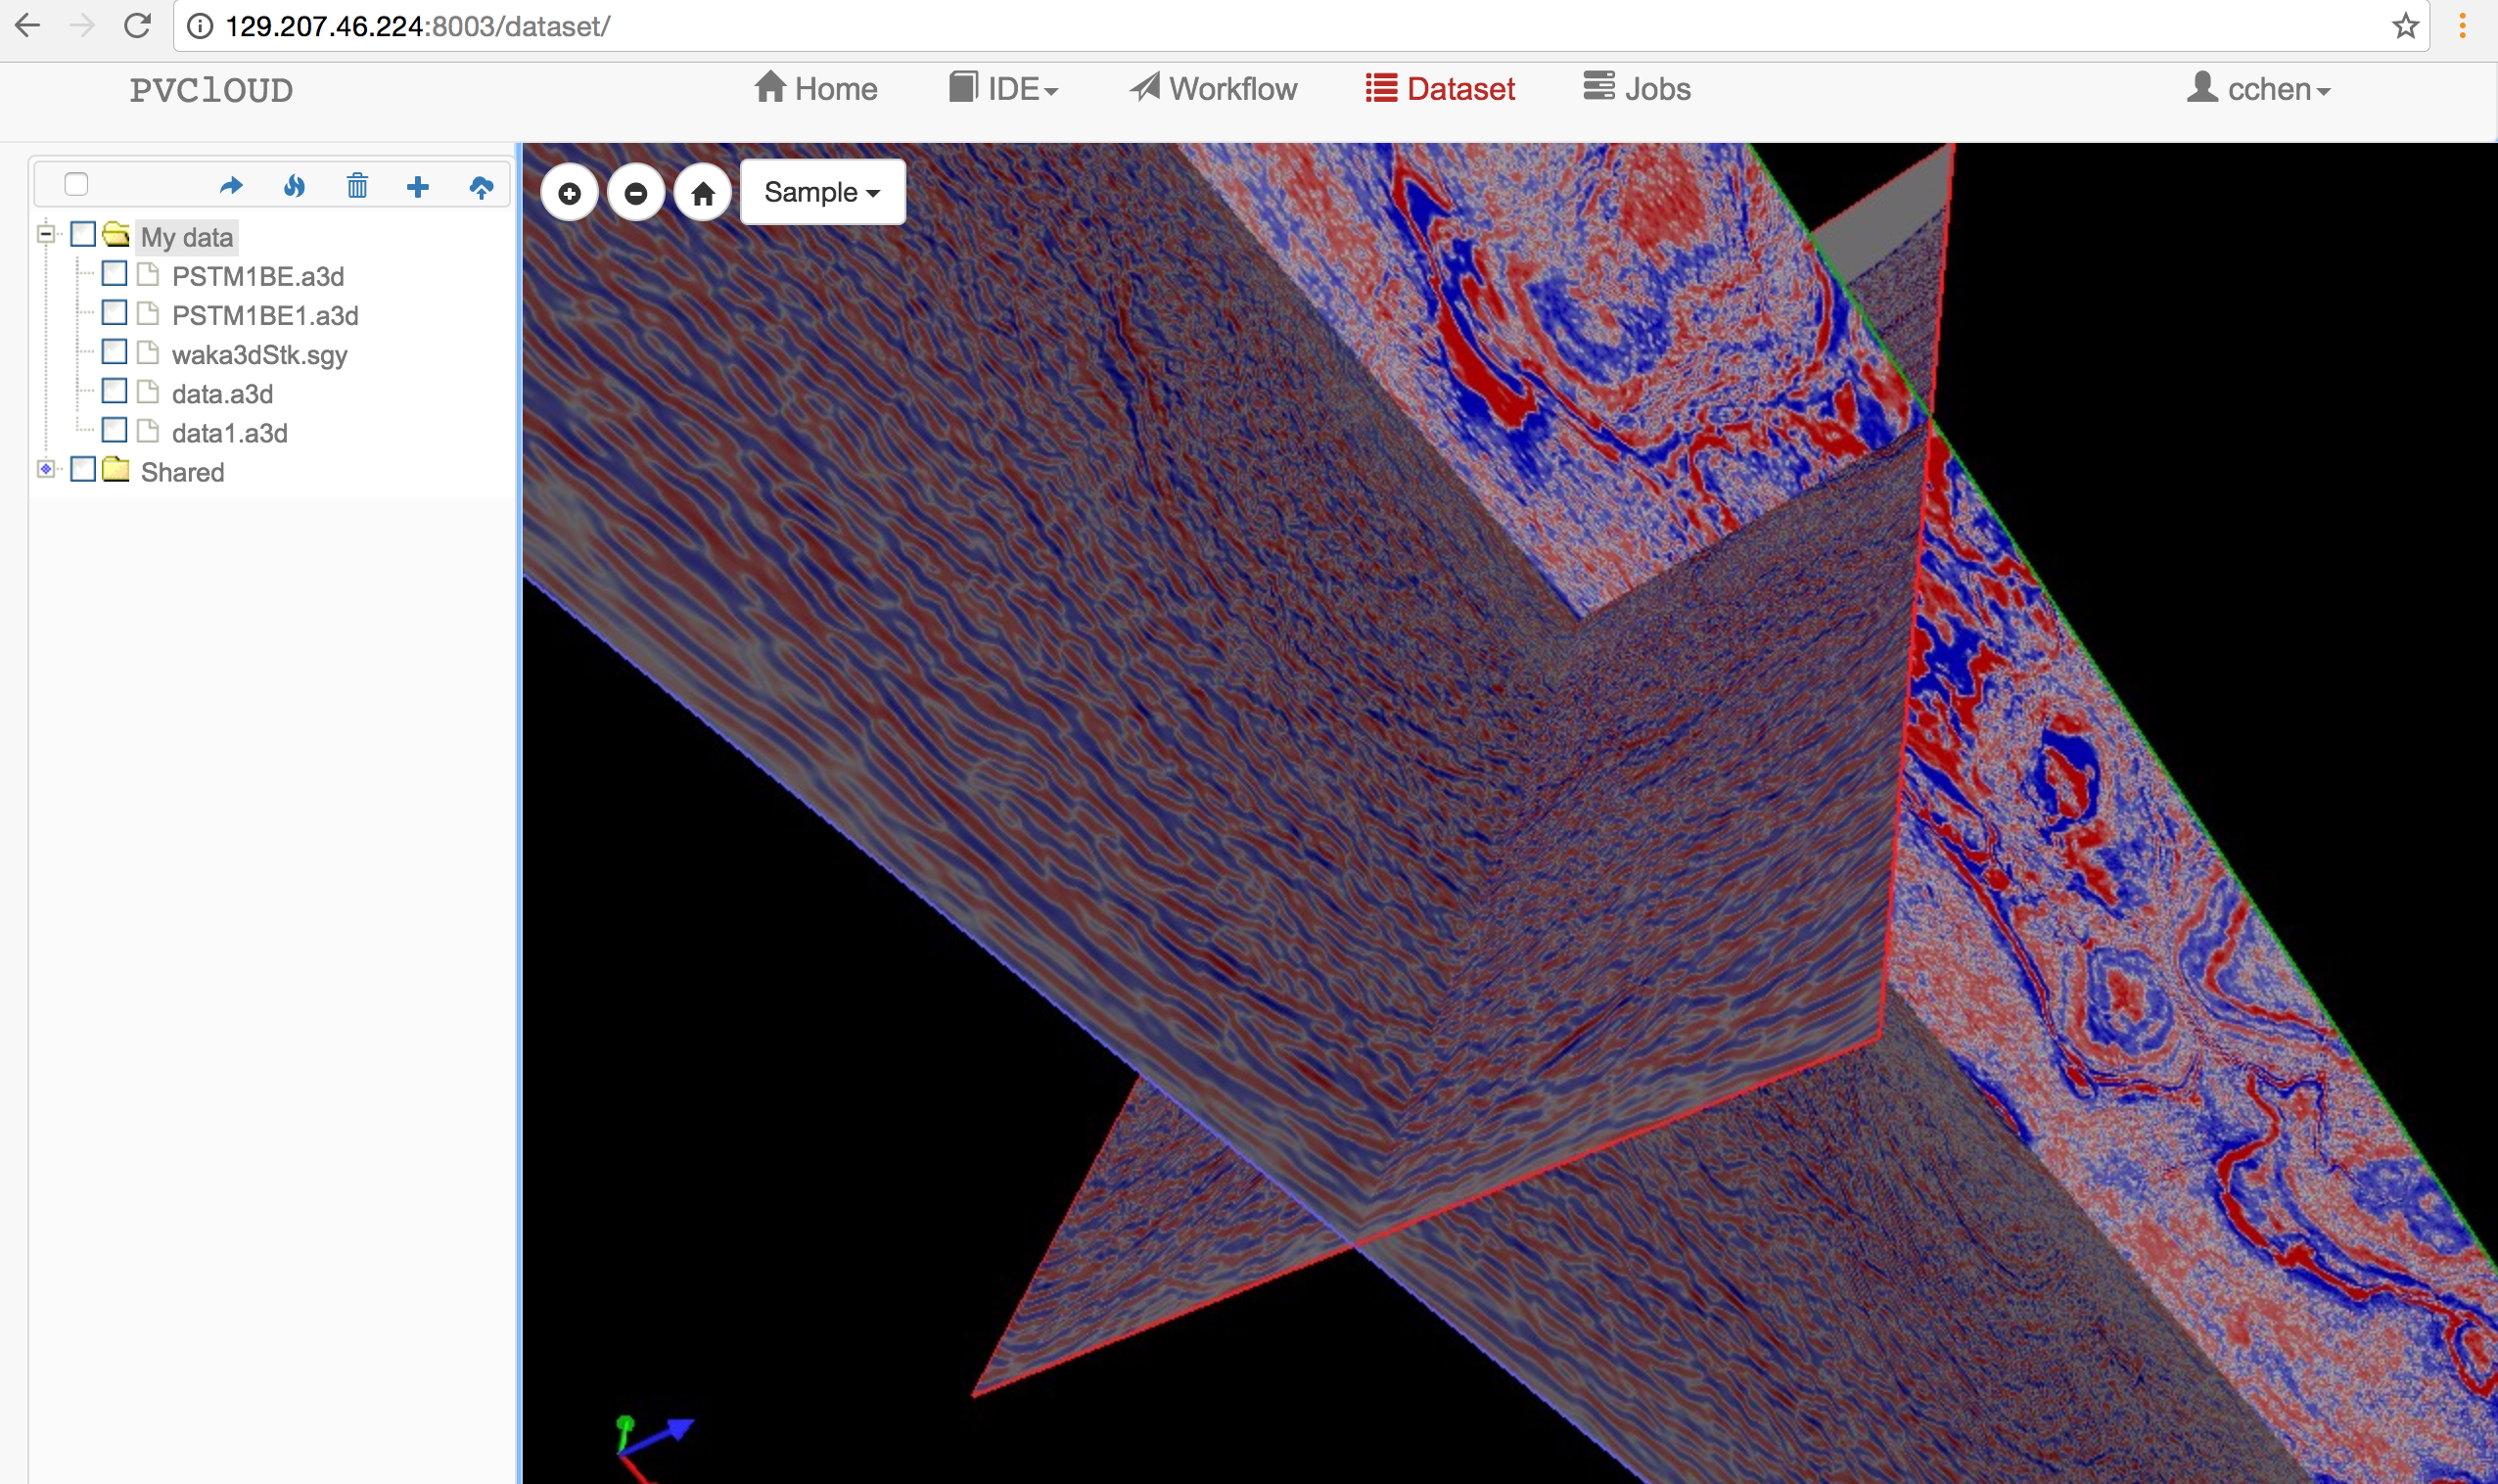
\includegraphics[scale=0.3]{figures/visualization.png}
\caption{Visualization Web Interface}
\label{visualization}
\end{figure}


\section{Web-based Workflow Platform}

Another service developed was a web-based workflow platform, which provides a user-friendly web interface to make cloud platform easy to use without programming, with which users could create workflow with drag and drop, could run the pre-built workflow and browse the results via the visualization service. This workflow web service was developed on top of the open-source project Clowdflows \cite{Clowdflows}, which provides a Django based web application framework to develop and manage customized widgets and workflows conveniently. As a free and open source web framework developed in Python, Django follows the classic Model, View and Controller (MVC) architectural pattern, so this application is suitable for interacting with both cloud service and web client.

The client side view of workflow is shown as Figure \ref{workflow}. Users could select widgets and specify seismic data files as input to construct their workflows. Each widget in the workflow view is an independent application component which could be implemented on top of Seismic Data Analytics SDK. A widget acquires at least one port as input or output thus multiple widgets are able to be combined to a workflow by multiple pipelines which connect the ports of all widgets. Each pipeline in the workflow view indicates a data communication, which transports data between widgets and drives the execution of whole workflow. The workflow framework implemented by Python code includes Django views (GUI), Django models (widgets data management) and topological sorting algorithm (connections check).  The data files are stored in HDFS of the cloud platform and could be browsed and selected from the navigation trees on the editor page.

\begin{figure}[h]
\centering
\includegraphics[scale=0.3]{figures/workflow.png}
\caption{Workflow Web Interface}
\label{workflow}
\end{figure}


%%%%%%%%%%%%%%%%%%%%%%%%%%%%%%%%%%%%%%%%%%%%%%%%%%%
%
%  New template code for TAMU Theses and Dissertations starting Fall 2012.  
%  For more info about this template or the 
%  TAMU LaTeX User's Group, see http://www.howdy.me/.
%
%  Author: Wendy Lynn Turner 
%	 Version 1.0 
%  Last updated 8/5/2012
%
%%%%%%%%%%%%%%%%%%%%%%%%%%%%%%%%%%%%%%%%%%%%%%%%%%%
%%%%%%%%%%%%%%%%%%%%%%%%%%%%%%%%%%%%%%%%%%%%%%%%%%%%%%%%%%%%%%%%%%%%%%
%%                           SECTION VI
%%%%%%%%%%%%%%%%%%%%%%%%%%%%%%%%%%%%%%%%%%%%%%%%%%%%%%%%%%%%%%%%%%%%%



\chapter{\uppercase{Conclusions and Future Work}}

\section{Conclusions}

In this paper, we focus on giving a friendly and high-efficiency solution to overcome the challenge of processing big seismic data. SAC was developed and verified with several typical applications, in which there is no prerequisite that users have parallel computing knowledge, and only the core algorithms need to be filled with the help of template provided by SAC. Such template provides friendly user interface for geophysicists without expense of performance. Some deep analysis about data partition, memory and network utilization are also given in this paper, which is a good experience for profiling any parallel program. From experiments and analysis results, SAC could handle big seismic data efficiently and easily. 

\section{Future Work}

Although SAC has been proved to be a good candidate for processing seismic data, there are still some other work to improve. Current templates could hand the basic applications, but for some complicate cases, more templates need to be defined. If an application has many reduce actions such as Jacobi stencil codes that could not run in pipeline in whole scope, the performance could not boost too much in parallel. It is still a challenge for defining template if worker thread need to communicate with each other, and we will follow Spark community closely to find a good solution for sharing data between workers. In the future work, we will add more templates to make them fit more applications. More high level machine learning algorithms should be added to SAC and be applied to more advance seismic models. To make SAC easy to be used by high level user and improve communication efficiency, workflow that could connect small piece of algorithms and Notebook for interactive seismic data processing are under development. Current visualization of seismic data in web interface is still in 2D mode, 3D view mode with remote rendering is already evaluated. For the performance optimization of parallel program in SAC, more deep research jobs are planned, such as adjusting GC parameters, GPU optimization and OpenSHMEM etc. In the view of applications developers, more data and computing models are need to investigate, such as streaming data, hybrid mode integrating with legacy codes etc. Fortunately, we had setup good relationship with many oil \& gas companies and related service companies through this project, and their requirements in applications will provide some right directions for our research. In summary, there is still a long way to go for solving big seismic data processing problems, but we are already on the way. 

%%%%%%%%%%%%%%%%%%%%%%%%%%%%%%%%%%%%%%%%%%%%%%%%%%%%%%%
%\begin{figure}[H]
%\centering
%\includegraphics[scale=.50]{figures/Penguins.jpg}
%\caption{Another TAMU figure}
%\label{fig:tamu-fig4}
%\end{figure}
%%%%%%%%%%%%%%%%%%%%%%%%%%%%%%%%%%%%%%%%%%%%%%%%%%%%%%%




%fix spacing in bibliography, if any...
%%%%%%%%%%%%%%%%%%%%%%%%%%%%%%%%%%%%%%%%%%%%%%%%%%%%%%%%%%%%%
\let\oldbibitem\bibitem
\renewcommand{\bibitem}{\setlength{\itemsep}{0pt}\oldbibitem}
%%%%%%%%%%%%%%%%%%%%%%%%%%%%%%%%%%%%%%%%%%%%%%%%%%%%%%%%%%%%%%%
\include{bibliography}
%\include{appendices}


\end{document}
